
\chapter{Functions (2 of 2)}

Like many things in life, writing functions is best learned by example. This
chapter will feature more of them that you can learn from and imitate.

\subsubsection{Basketball scoring: \texttt{bb\_pts()}}

Continuing the sports theme, the total points a basketball player scores is
related to the number of shots she makes of various kinds. Typically, the ``box
score'' of a game (see example in Figure~\ref{boxScore}) reports three scoring
stats: (1) the \textit{total} number of ``field goals''\footnote{A ``field
goal'' in basketball just means ``a regular basket'' -- \textit{i.e.}, not a
free throw penalty shot.} a player made and attempted, (2) the number of these
field goals, if any, that were for three points\footnote{In most leagues, a
basket is worth 2 points unless the shooter was farther than a certain distance
from the hoop when she shot it, in which case it's worth 3.}, and (3) the
number of free throws (``easy'' penalty shots) the player attempted and made.

Confusingly, (1) \textit{includes} (2). In other words, if the first number is
4 and the second is 1, the player didn't score 4 regular two-point baskets and
1 three-pointer, but rather \textit{3} two-point baskets and 1 three-pointer.

\begin{figure}[ht]
\centering
\fbox{
\mbox{
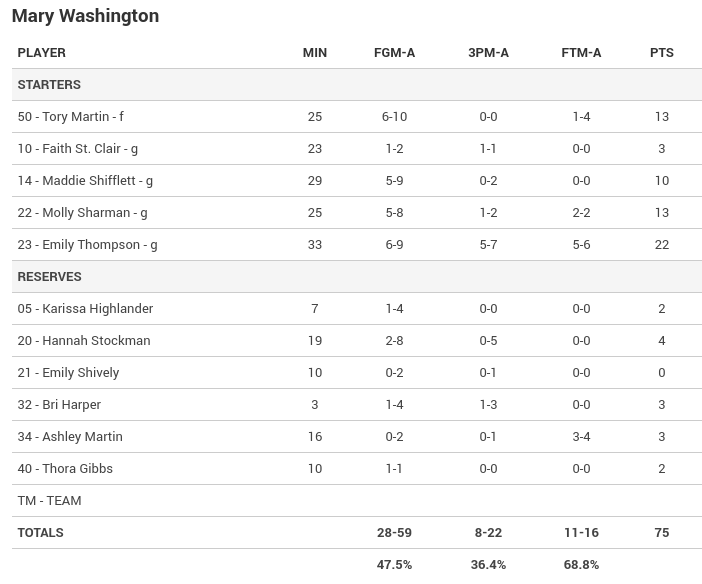
\includegraphics[width=0.8\textwidth]{boxScore.png}
}
}
\medskip
\caption{A basketball box score.}
\label{boxScore}
\end{figure}

In Figure~\ref{boxScore}, the \textsf{FGM-A} column gives the first of these
three categories, \textsf{3PM-A} the second, and \textsf{FTM-A} the third. The
\textsf{PTS} column gives the total number of points that player scored. (For
example, Molly Sharman made 5 of her 8 attempted field goals, one of which was
for three points, and she also converted both free throw attempts.)

All that took a lot longer to explain than the corresponding Python function:

\begin{Verbatim}[fontsize=\small,samepage=true,frame=single,framesep=3mm]
def bb_pts(fgm, threep_fgm, ftm):
    return ((fgm - threep_fgm) * 2) + (threep_fgm * 3) + (ftm * 1)

torys_pts = bb_pts(6, 0, 1)
print("Tory scored {} points.".format(torys_pts))
print("Emily scored {} points.".format(bb_pts(6, 5, 5)))
print("The Lady Eagles scored {} points!".format(bb_pts(28, 8, 11)))
\end{Verbatim}
\vspace{-.2in}

\begin{Verbatim}[fontsize=\small,samepage=true,frame=leftline,framesep=5mm,framerule=1mm]
Tory scored 13 points.
Emily scored 22 points.
The Lady Eagles scored 75 points!
\end{Verbatim}

\index{PEMDAS}

Strictly speaking you don't need all those bananas (regular PEMDAS
order-of-operations applies) but I think it's a good idea to include them for
clarity and grouping.

% any_zeros()
% quiz_avg()
